%
%\documentclass[referee]{aa} % for a referee version
%\documentclass[onecolumn]{aa} % for a paper on 1 column  
%\documentclass[longauth]{aa} % for the long lists of affiliations 
%\documentclass[letter]{aa} % for the letters 
%\documentclass[bibyear]{aa} % if the references are not structured 
%                              according to the author-year natbib style


\documentclass{aa}  
\usepackage{hyperref}
\usepackage{graphicx}
%%%%%%%%%%%%%%%%%%%%%%%%%%%%%%%%%%%%%%%%
\usepackage{txfonts}
\usepackage{multirow}
%%%%%%%%%%%%%%%%%%%%%%%%%%%%%%%%%%%%%%%%
\usepackage{subcaption}

  % results heading (mandatory)
\begin{document} 


   \title{Data processing pipelines and the data center for the X-ray spectrometer/imager STIX}

   \subtitle{}

   \author{Hualin Xiao
          \inst{1}
          \and 
          Shane Maloney 
          \inst{2}
          \and S\"am Krucker\inst{1}
          \and Paolo Massa \inst{6}
          \and Lastufka Erica \inst{1}
          \and Andrea Francesco Battaglia\inst{3}
          \and Ewan Dickson \inst{4}
          \and Frederic Schuller \inst{7}
          \and André Csillaghy\inst{1} 
          \and Ryan Daniel \inst{1}
          \and László Etesi \inst{1}
          \and Nicky Hochmuth \inst{1}
          \and Collier Hannah \inst{1}
          \and Gordon Hurford\inst{1} 
          \and Olivier Limousin \inst{5}
          \and Astrid M. Veronig\inst{4} 
          \and Alexander Warmuth \inst{7}
         }

   \institute{University of Applied Sciences and Arts Northwestern Switzerland (FHNW), 5200 Windisch, Switzerland \\
              \email{hualin.xiao@fhnw.ch}
         \and
          Astrophysics Research Group, School of Physics, Trinity College Dublin, Dublin 2, Ireland
          \and
             ETH Z\"urich, R\"amistrasse 101, 8092 Z\"urich, Switzerland
         \and University of Graz, Universitätspl. 3, 8010 Graz, Austria
         \and IRFU, CEA, Université Paris-Saclay, and Université Paris Diderot, AIM, Sorbonne Paris Cité, CEA, CNRS, 91191 Gif-sur-Yvette,
         France
         \and Dipartimento di Matematica, Università degli Studi di Genova, Via Dodecaneso 35, 16146 Genova, Italy
         \and Leibniz-Institut für Astrophysik Potsdam (AIP), An der Sternwarte 16, D-14482 Potsdam, Germany
             }

   \date{}

% \abstract{}{}{}{}{} 
% 5 {} token are mandatory
 
  \abstract
  % context heading (optional)
   {} %leave it empty if necessary  
  % {context.}
  % aims heading (mandatory)
   { The Spectrometer/Telescope for Imaging X-rays (STIX) instrument onboard the Solar Orbiter mission launched on February 10,
    2020 promises advances in the study of solar flares of various sizes. 
    It is capable of measuring X-ray spectra from 4 to 150 keV with 1 keV resolution binned into 
    32 energy bins before downlinking. STIX data center is an infrastructure established at FHNW.
    It purposes include  processing and archiving STIX data, supporting 
    operations of the instrument and providing data and tools to the solar physics community.
    It consists of databases and automated data processing pipelines, various tools for data analysis. 
    The automated data processing pipelines turn raw telemetry data into processed information and data products. 
    Processed information and data products are archived at the data center.  
   }

   {Results.}
  % conclusions heading (optional), leave it empty if necessary 
   {}

   \keywords{Solar flares --Data Center --
                STIX data products --
                Data processing pipeline
               }

   \maketitle
%
%-------------------------------------------------------------------

\section{Introduction}
Solar Orbiter is a Sun-observing mission of the European Space  Agency that 
addresses the interaction between the Sun and the heliosphere.
It was launched on Feb. 10, 2020 for a nominal mission duration of seven years and a planned 
extension of
three years. It carries ten sets of instruments for comprehensive
remote-sensing and in-situ measurements. 
Solar Orbiter  will perform detailed measurements of the Sun as close as 0.28 AU and for the first time look at its uncharted polar regions (\cite{SolarOrbiter2020}).  
Its goal is to  address the center question of heliophysics  "How does the Sun create and control the heliosphere?".  It is designed to identify the origins and causes of the solar wind, the heliospheric magnetic field, the solar energetic particles, the transient interplanetary disturbances, and the Sun's magnetic field.
This consists of the study of energetic solar phenomena like flares,  solar transients,  the solar wind accelerating mechanisms, and the solar dynamo principle.  
The Spectrometer Telescope for Imaging X-rays (STIX) is one of the ten instruments onboard Solar Orbiter.  
It measures X-rays from 4 to 150 keV and takes X-ray images with a few arcsec angular resolution by using an indirect imaging technique,
based on the Moiré effect.  STIX consists of 32 collimators with grids and pixelated Cadmium telluride detector unit Caliste-SO. 
The main science objective of STIX is to study the extremely hot solar plasma and the high-energy electrons accelerated during solar flares. STIX provides  intensity,  spectrum, timing, and location of accelerated electron information of solar flaresn.
For details on STIX instrumentation and its scientific capabilities, we refer to the instrument paper (\cite{StixInstrument}).


During nominal science operations, STIX continuously acquires data. They are compressed and formatted into different types of telemetry packets onboard by 
STIX onboard data processing unit (IDPU). The total number of telemetry packets reaches hundreds. 
Being aware of the complexity of STIX data analysis and  the need of bringing the data to the solar physics community, 
a data center was developed at FHNW. 
The data center software consists of a set of software packets, which allow 
The data center (SDC) receives, analyzes, archives and distributes STIX data. 
It also supports STIX in-flight operations.
It turns raw telemetry data into processed information and produces data products that can be used for scientific analysis.
It also provides various data visualization tools to the solar physics community.
The purpose of this paper is to describe the processing pipelines, 
the main algorithms of automated data processing, data products and tools provided by the STIX data center.
%We will describe here STIX data types,  the flow of data from to the users, the data processing pipelines, the %database, the data products and the tools provided for the solar physics comnunity.
%--------------------------------------------------------------------
STIX data center processes STIX telemetry to generate a set of widely usable products, as well as performing a quick-look
analysis to access the data quality and discover solar flares. Data are distributed to users and archived at STIX data center. 
STIX data center also provides various data analysis tools, and giving support to users. 

This paper is organized as follows: Section \ref{sec:raw-data} briefly introduces STIX raw telemetry types, data flow and
telemetry processing pipelines. 
At the end it is a summary \ref{sec:summary}.
\section{STIX raw telemetry data}
\label{sec:raw-data}
STIX continuously observes high-energy events on the Sun at 4 -- 150keV. 
Photons emitted by solar flares are detected with 32 subcollimators 
(a 12-pixel-detector behind a front and rear grid). While passing through the front and rear grids, 
the flares generate a modulation pattern over the 12 pixels of each detector. 
The pattern can then be used to reconstruct images and to do spectroscopy. 
Other data products include lightcurves, flare information, spectra, and background information.
The nominal telemetry budget of STIX is 50 bps.
STIX is far from earth, not all data can be downloaded from the spacecraft. We have low latency data.
For bulk science data have to be requested.
STIX continuously collects energy deposition information from 32 detector units, the aspect system,
and engineering sensors in the nominal observation mode.
The collected data are first processed by the FPGA and the onboard flight software
After the prompt processing, low latency telemetry data are directed to the
storage in the spacecraft whereas high time resolution pixel data are written to STIX onboard archive memory for
later processings.
STIX transmits data to the spacecraft in the form of binary packets.
STIX raw telemetry data can be classified into four
categories: housekeeping data, diagnostic data, quick-look data and science data.

In the next sections, we briefly introduce the main raw telemetry data types.
For details about STIX raw telemetry data, we refer to STIX instrument paper (\cite{StixInstrument}).

\subsection{Housekeeping data}
 %\item  Housekeeping data.
 %STIX generates two different houskeeping data packets.
STIX housekeeping data (HK) contain engineering data that measure temperatures, voltages, currents, the status of switches,
averaged signal readouts from the four photodiodes in the aspect system, detector trigger counts, and the flags indicating
status bits of the onboard software and the archive memory.
The data is used to monitor instrument status, and the instrument pointing.
%All the parameters are reported in the same type packet at a fixed 64 sec cadence.
HK data are generated as long as STIX is powered on.
During nominal operations, a housekeeping packet is generated every 64 seconds, which results in a daily raw telemetry of  143 kiB.
All STIX sensors and the IDPU will produce housekeeping data that will be received on the ground with the highest priority
for monitoring instrument status and health.

\subsection{Quick-look data}
STIX has only one operational mode in which Low Latency data is produced, and that is  NOMINAL mode, which is the regular science mode.
STIX generates four different types of quick-look (QL) data:
\begin{itemize}
%of all pixels in 30 detectors (excluding background detector and the coarse flare locator)
%accumulated every 4 sec time resolution in five broad energy ranges (two thermal, two nonthermal
%and one intermediate). Quick-look light curves are generated when STIX is in nominal observation mode.
\item STIX quick-look light curves. 
STIX quick-look light curves are time series of detector-sumed counts in five energy bands, with a default integration time of 4 seconds. 
Counts are not corrected for dead time,  transmission, impacts of the presence of the attenuator  or rate control regimes. 
STIX quick-look light curve data are transmitted to the ground as other low latency data. 
Typically, STIX data centers receive them within tens of minutes to two days after being generated on board.
% efficiency. The FITS file is in accordance with [LLFITSICD] but will also comply with  in order to be usable with existing high-energy solar data file routines.
%The light curve data are structured as an array of five count values COUNTS (for the five energy bands) 
%per time, where time is a relative time $RELATIVE_TIME$ since $OBT_START$ that is time bin centered (i.e. with an integration 
%time of 4s, $RELATIVE_TIME$ will 2-6-10…, as opposed to 0-4-8…). It is possible that 
% $RELATIVE_TIME$ “jumps”, e.g. when the attenuator is moving in and the affected time bin 
% becomes undetermined and is left out. Additionally, there is an energy channel reference 
% CHANNEL, with indices into the energy axis in the second extension. Given below is an I
% DL-based structure notation.
\item Background monitor light curves. Background monitor light curves are similar to the Quick-look light curves but only
counts recorded by the background detector pixels are included, and the integration time is 8 seconds.
\item Variance data are onboard computed variance of 40 successive detector-summed count rates
based on 0.1 sec integration.
\item Quick-look spectra, which are energy snapshots of energy spectra (32 science energy bins) for
each of the 32 detectors with 32 sec exposure time.
STIX takes a snapshot of energy spectra every 1024
seconds in the nominal observation mode.
\item Calibration spectra. Calibration spectra are accumulated for events from 128 weak onboard $^{133}$Ba radioactive sources 
(a total activity of 4500 Bq) 
 when the solar count rate is small compared to the background.
Identification of such quiet periods is done autonomously, based on the presence of a
TC-specified time gap between two successive photons.  
ADC readouts of each channel are accumulated in individual spectrum.
After an accumulation a long period (typically 24 hours),  the spectra are 
formmated and redirected to in the quick-look low-latency data.
\end{itemize}
\subsection{Diagnostic and event data}
When a failure is detected directly by STIX, the instrument’s response includes sending a
“dedicated” telemetry event report with appropriate diagnostic information included.

\subsection{Bulk science data}

Bulk science data are different combinations of summing and compression of the basic pixel data stored in STIX onboard archive memory, which can be used for spectrocopy and imaging.
To cope with the limited available telemetry, they are not automatically included in the telemetry.
Onboard formation of the science data is invoked by data request telecommands.
Each science request can select subsets of energies, pixels and detectors.
Six different science data can be generated:
\begin{itemize}
 \item Raw pixel data is the least processed data and contains uncompressed counts for the selected energies, pixels and detectors;
\item Pixel data is essentially the same as Level-0 but the counts are compressed onboard before being sent to the ground;
\item Compressed pixel data are further compressed counts from the L1 pixel data, in which are summed down to 4 before compression.
\item Visibilities are further reduces the data by combining the four summed pixel counts into complex visibility which is also compressed.
\item Spectrograms are detector summed spectrograms;
\item High-time resolution aspect data.
\end{itemize}
It should be noticed that the data levels described 
above are on-board data levels. They are sent to the ground in the format of raw binary packets and 
considered as level-0 at STIX data center.  
\begin{table}[h]
\centering
\caption{STIX raw telemetry data coverage, data rate and typical reception delay at SDC.  }
\resizebox{0.8\linewidth}{!}{
\begin{tabular}{lllll}
\hline
Category &  Coverage &Daily data volume & Reception Delay  \\ \hline
Housekeeping           & continous &   143 kiB  & hours to days \\ \hline
Quicklook     & continous         & $\sim$ 358 kiB  & hours to days   \\ \hline

Science     & ground-selected only &  $\sim$ MiB to $\sim$ 10 MiB &  2 to 12 weeks   \\ \hline
Calibration  & quiet sun periods  & 100 kiB  & $\sim$ 1 day \\ \hline
\end{tabular}
}
\label{tb:raw_types}
\end{table}

Housekeeping data, quick-look data and calibration data are directed to the
common low latency data stored in SSMM in the spacecraft.
The coverage, data rate and latency of 
different types of STIX raw telemetry data are
summarized in Table \ref{tb:raw_types}.

%https://issues.cosmos.esa.int/solarorbiterwiki/display/SOSP/SOC+Archive+Plan?preview=%2F11734040%2F21759347%2FSOL-SGS-PL-0009-SOARPL-2.0.pdf

\section{Data reception}

During nominal science operations,
Low latency data are down-linked in the very next ground station pass regardless of orbital geometry, 
whereas science data are only down-linked when the bandwidth permits.
The downloaded instrument telemetry data are first processed by ESA's ground segment
software at the Solar Orbiter mission control center. Then they
are distributed to instrument teams by the ESA EGOS Data
Dissemination System (EDDS) (\cite{EDDS}) according instrument teams' preset conditions.

Telemetry data received by STIX data center from EDDS  are in the binary format, and have the same
 information content as the original telemetry generated by STIX.
The low-latency data arrives at STIX data center with delays ranging from a few minutes to a few days, depending on whether there
are antenna passes, whereas science data may arrive several weeks after being generated onboard.

In addition to the telemetry data, STIX data center also receives SPICE kernels (\cite{spice1996,spice2018})  from the science operations center.
They contain information of spacecraft ephemeris and clocking calibration factors required for time conversions.


\section{Data processing pipelines}
\subsection{Data processing pipeline overview}


\begin{figure*}
    \centering
    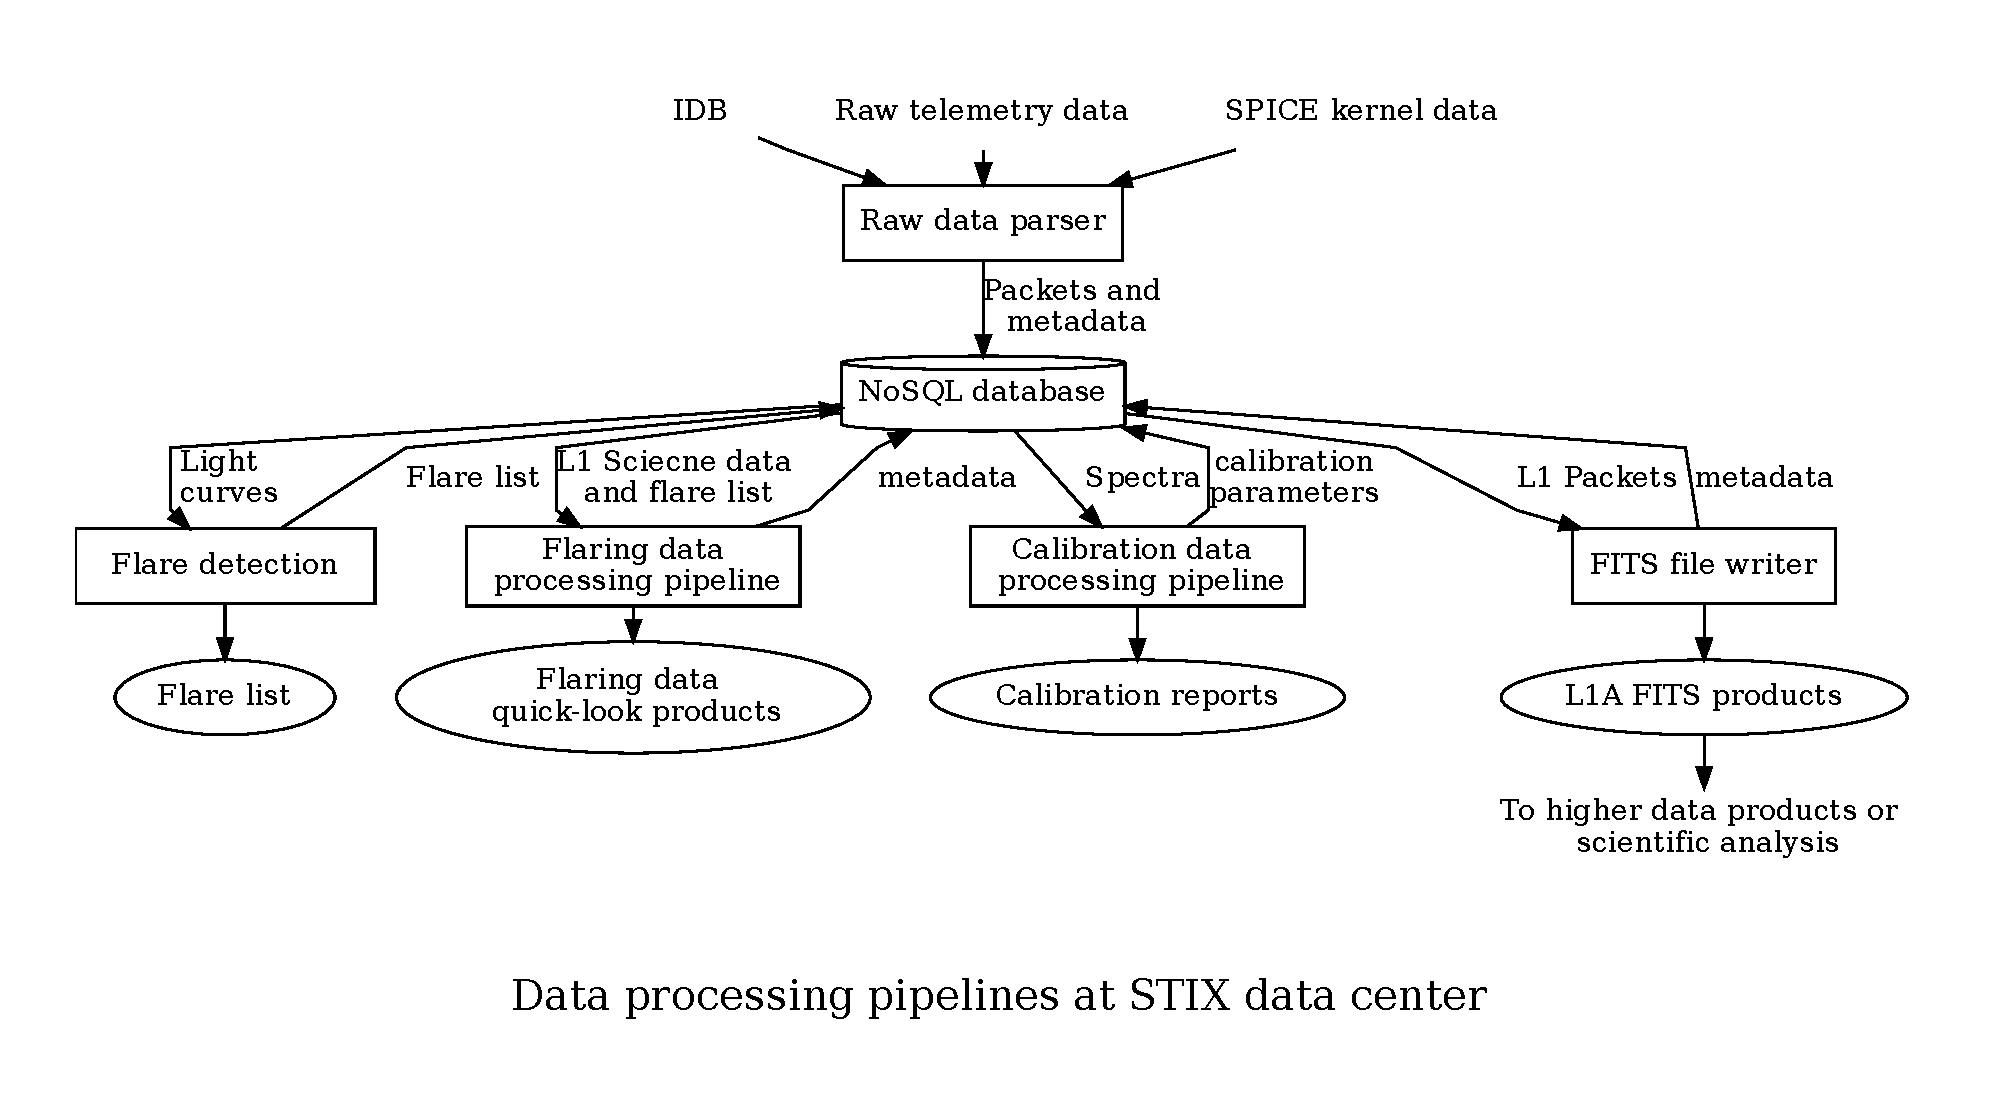
\includegraphics[width=0.9\textwidth]{figures/pipelines.pdf}
    \caption{Data processing pipelines at STIX data center.}
    \label{fig:main_pipelines}
\end{figure*}
New telemetry data arriving at STIX data centers is immediately processed by the pipelines as shown 
in Fig. \ref{fig:main_pipelines}. 
The processing is started from raw packet parsing. Parsed level-1 packets are written to a NoSQL database. 
Then they are selected  are processed in 4 different paths, 
In the first path,  housekeeping, quick-look and science packets 
are selected and used to create L1-A FITS files, 
which can be used for scientific analysis. 
The second path selects calibration data from the database and extracts energy calibration factors for 
instrument monitoring. In the third path, quick-look packets are selected and used to identify solar
flares; The fourth path processes flaring data, 
generating higher data products.   

\subsection{Raw data parsing and database}
New telemetry data arrived at STIX data center are immediately processed by STIX data parser, 
which is capable of parsing all types of STIX binary telecommands and telemetry packets.   
Parsing of packets is based on the mission interface database (MIB), which 
contains information on packet parameters such as names, descriptions, lengths,
data types. The parser extracts header and parameters for each raw binary packet
using the information in the MIB.
Packets after parsing contain raw values of parameters. 
 Spacecraft clock times are further converted to UTC times using 
the latest version of SPICE kernel data (\cite{spice1996,spice2018}), compressed integers are  
decompressed by using a LUT table and 
housekeeping raw values are converted to 
human-readable values using the calibration factors or look-up tables stored in the MIB. 
Packets after the above processing steps are called level-1 packets. They
have tree structures, each containing two nodes "header" and "parameters";
the former contains the basic information  of the packet such as timestamp, packet type,
and the latter contains names, 
raw values, engineering values (or decompressed integers) and child nodes of a list of parameters.
Level-1 packets are written 
to a NoSQL database. 
NoSQL database is schemaless,  making it ideal to store data with complex
structures but small sizes like STIX level-1 packets.  
NoSQL is also 

In addition to packets, the NoSQL also stores other data extracted by the parser during packets parsing, 
for example, 
\begin{itemize}
  \item Raw file metadata. It contains filename, reception time, observation start time and stop time, MIB and SPICE kernels used by the parser ; 
  \item Bulk science metadata, which contains the observation time range, detector and pixels masks, energy ranges, 
   bulk science data types, and IDs of packets in the database; 
  \item Quick-look light curves.  The dataset contains data of counts, time range, energy bins extracted from QL LC packets, 
     allowing for  quick access to QL data with web pages or APIs;
  \item STIX instrument configurations. 
  It contains the instrument configuration parameters for such as  energy conversion factors and AISICs, 
  allowing fast tracking of the instrument settings;
\end{itemize}
The information are necessary for subsequent processing. The
database is  accessible through web pages at STIX data center website or python APIs. 
\subsection{Data products}
\subsubsection{Level-1 FITS files}
After each new raw telemetry file is being parsed, 
housekeeping, quick-look, and science packets  
are selected from the NoSQL database successively 
and checked for data integrity and consistency. 
Then packets of the same type are merged for creations of pre-release of 
level-1 data products (Level-1A) 
 in the FITS format (\cite{fits}), 
which is a portable file standard widely used in the astronomy 
community to store images and tables.
It should be noted that the data levels mentioning here are data processing levels. 
In order not to confuse two conventions, we use different notations to indicate onboard level in this paper. 
Metadata such as observation time range, creation time, filenames,  checksum are written to 
the primary header data units (HDU) of fits files. 
They are also written to a dataset in the database.

Level-1A FITS files are generated automatically and available at STIX data center within minutes 
after the reception of a raw file.
It should be noticed that predicted SPICE kernels may be used when the reconstructed spice kernels  
are not available, and the L1A data are subjected to some known issues 
due to bugs in the early version of the flight software.
After all resources are validated,  Level-1  FITS files are created again. 
Level-1  FITS products have almost the same data structures as Level-1A.
\subsubsection{Level-2 FITS files}
Level-1 FITS files are further processed. 
Dead time  correction and energy this make up the second
\subsubsection{Level-3 data products}
Level-3 data products are visibilities and images

\subsection{Energy calibration}
Energies deposited by x-rays are converted from ADC units 
to keV onboard by using an energy look-up table (ELUT),
 which is regularly updated  with telecommands.
ELUTs can be constructed using energy conversion factors obtained by studying
positions of photo peaks in the calibration spectra measured for the onboard Ba$^{133}$ sources.  
As energy conversion factors may change with temperature 
or polarization effects,  calibration spectra need to be analyzed promptly on the ground. 

\begin{figure}
 \centering
  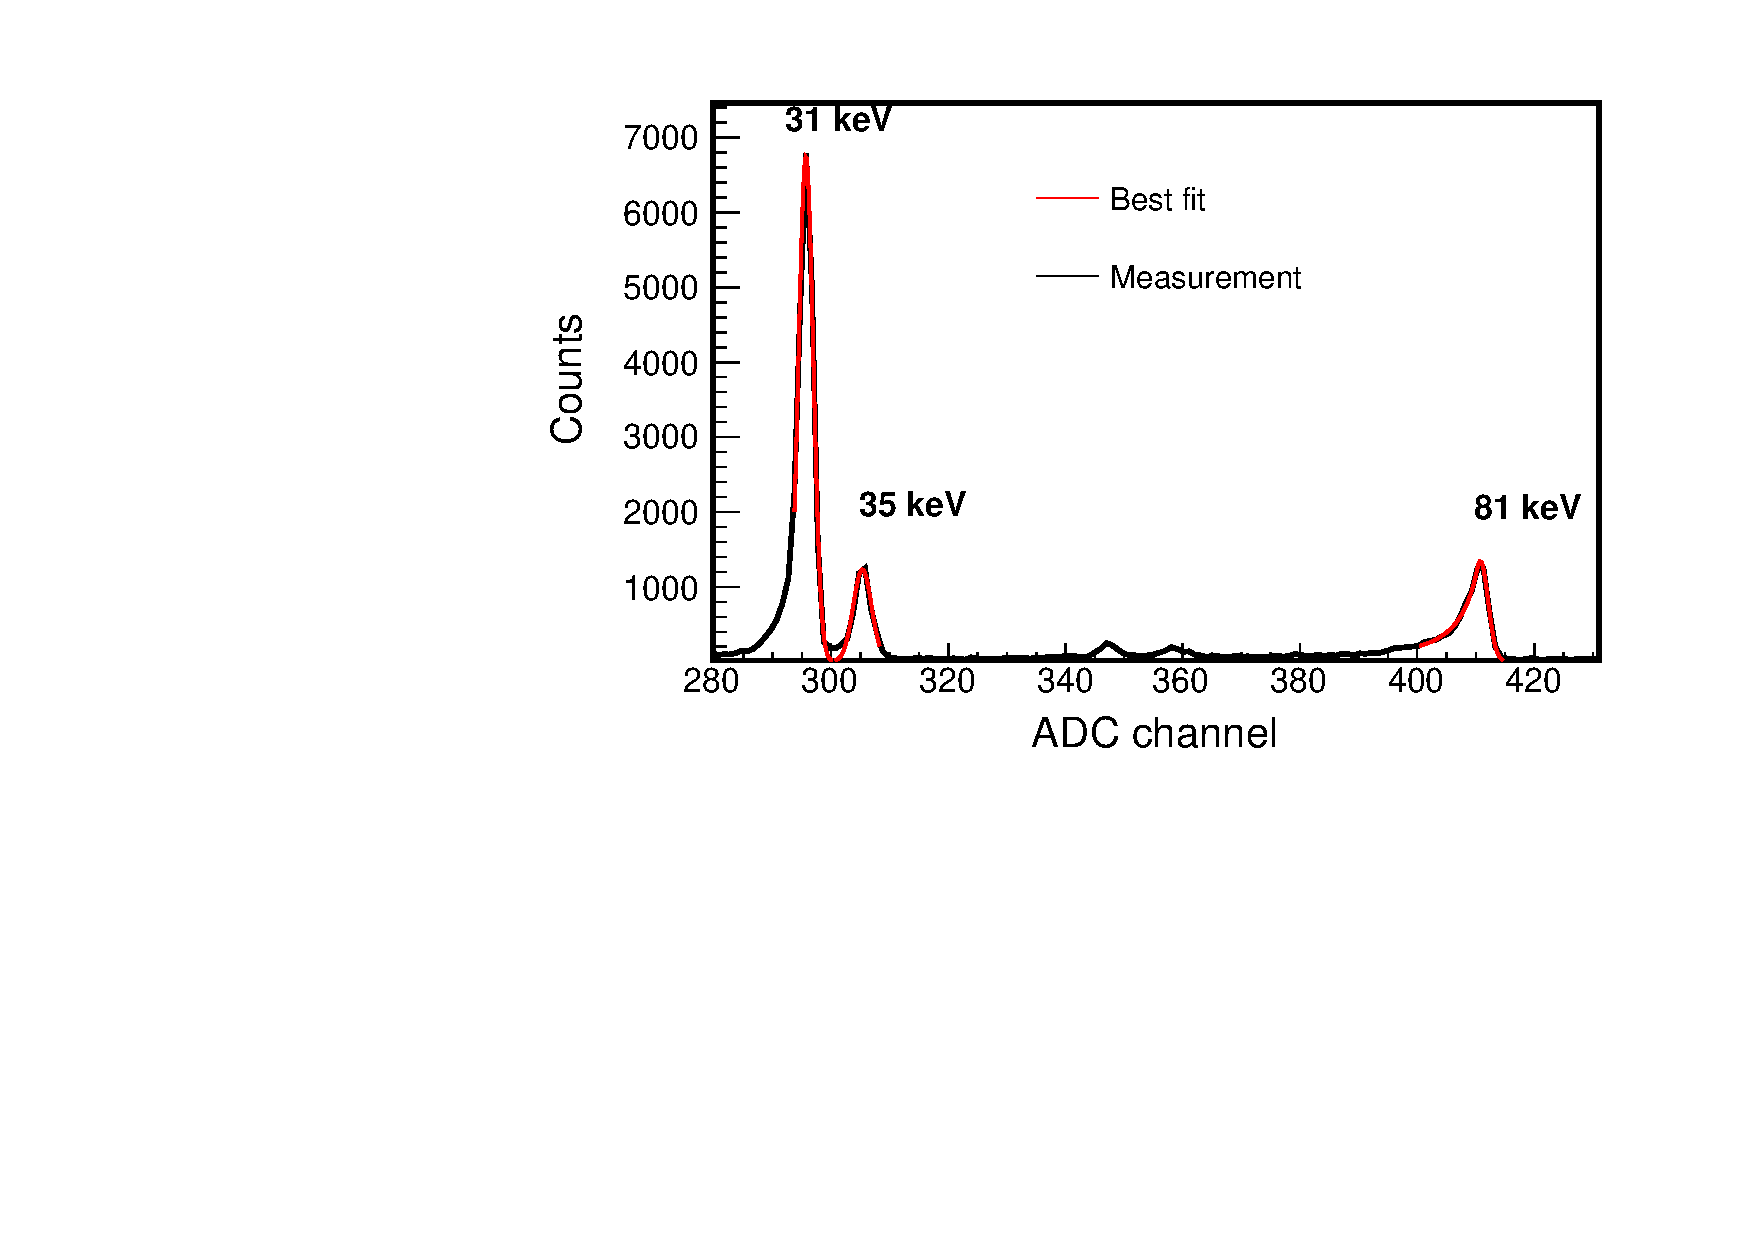
\includegraphics[width=0.8\linewidth]{figures/cal-fit.pdf}
  \caption{An example of STIX in-flight calibration count spectrum.
  The three strongest lines, from left to right, are from 31 keV, 35 keV, and 81 keV
  photons. The first two peaks are fitted by the double-Gaussian function and the high energy peak by  
  the crystal-ball function. }
    \label{fig:cal-fit}
\end{figure}
The right panel of Fig.~\ref{fig:cal-fit} shows 
an example of STIX count spectrum from in-flight calibration run.  
The three strongest lines are from 31 keV, 35 keV and 81 keV photons. 
The first two peaks are fitted with the double-Gaussian function and the third peak
by the crystall-ball function (\cite{crsystallball}),  which consists of a Gaussian core portion 
and a power-law low-end tail, below a certain threshold.
Then a linear line is fitted to the relation between
the three fitted peak positions (in ADC unit) and the photon energies in units of keV.  
The interception and slope indicate the baseline and gain of the channel. 
The results were compared to those determined using the ECC method (see \cite{ecc,ecc2})), 
 which were found to be consistent within errors.
The above steps are performed for each calibration run automatically 
once the data is available at STIX data center.  The results are written to a
 dataset in  NoSQL database.  It is accessible through a web page at STIX data center or python APIs.

Calibration factors are monitored continuously. Once significant changes are 
observed from those used for the construction of  the onboard ELUT, 
 a new ELUT is  created and  then uploaded to STIX after being validated by the operations team. 

\subsection{Solar flare identification}
The in-flight software identifies solar flares by comparing  the count rate of 
the background detector with that of other detectors 
 and packs the results into the QL flare flag and location reports.
However,  the reports only provide limited information on flares due to the constraints of telemetry 
bandwidth and the limitation of onboard computing resources, and micro-flares are not 
reported due to the relative high trigger threshold.
Using QL light curves, solar flares can be identified on ground in great detail.

QL light curves of the energy range from  4 to 10 keV are used for solar flare identification
on the ground. Identification is based on the fact 
that the background event rate in that energy range is almost constant 
over a timescale of days during quiet sun periods. 
The procedure involves the following steps:
\begin{itemize}
  \item Light curve smoothing. The selected light curve is filtered using an unweighted
  moving average filter with a time window of 1 minute to smooth out statistical fluctuations and electric surge spikes;
  \item Identification of flare peaks. Peaks with counts exceeding a threshold of $2\sigma$ above the background level
   are selected. The duration of a peak is given by the time difference between the first 
   crossing of the threshold on the left and right sides of the peak;  
  \item Merging of flare peaks. If the time difference between the two peaks is less than 5 minutes,
   they are considered to be from the same flare.
\end{itemize}

\begin{figure}
  \centering
  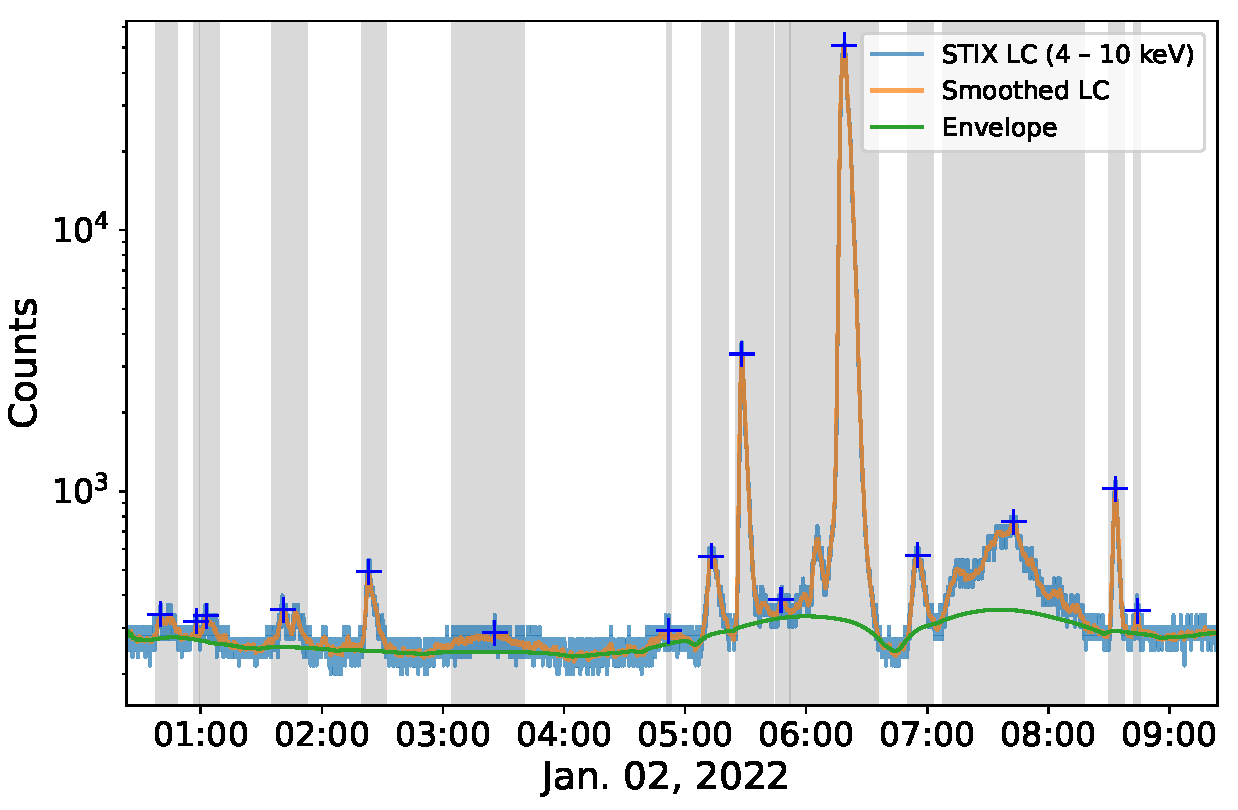
\includegraphics[width=0.8\linewidth]{figures/flaredet.pdf}
  \caption{STIX 4 -- 10 keV QL light curve recorded from 2022-08-10T21:00:00Z to 2022-08-10T18:00:00Z and 
  identified flares.   
  The light curve was smoothed using a moving average filter with a time window
  of 1 minute. 
  The identified peaks are marked with plus signs, and flare time ranges are colored in cyan.
  }
  \label{fig:flare-det}
\end{figure}
As an example, Fig.~\ref{fig:flare-det} shows  the 4 -- 10 keV QL  light curve recorded from 
2022-08-10T10:00:00Z to 2022-08-10T18:00:00Z,
 as well as the smoothed light curve and  identified solar flares (marked with plus signs).

For each identified solar flare,  start time, end time, peak time and peak 
counts are extracted from the selected light curve and assigned 
an 8-digit identification number of the format yymmddHHMM, which represents the solar flare peak time. 
For example, the identification number 2201010000  indicates that 
the solar flare peak time is at 2022-01-01T00:00:00 UT. 
The above steps are repeated  for the QL light curves of other four higher energies
in the same time frame. This can provide information on the upper limit of the X-ray energy produced by the flare,
which is used to optimise the selection of scientific data to be downloaded. 
Then all extracted information as well as the ephemeris data calculated for the peak time are 
written to a dataset called solar flare list in the NoSQL database.
The flare list database can be queried using web interface or stixpy.
\subsection{Estimation of background level}
As mentioned earlier, a threshold value calculated using background data needs to be provided when
performing flare identification.  
The background, although stable within a few days, can change over long periods of time,
 a suitable threshold is important for the accuracy of the identification. 
 Therefore, QL light curves for  quiet sun periods are selected by excluding flaring periods. 
 Then median values and variances are calculated from the selected light curves and 
 written to a dataset in the database. They are used as inputs of the next flare identification. 
 Those processing steps are performed automatically after flare identification.

\subsection{Solar flare data analysis pipeline}
\subsubsection{GOES class determination}
\begin{figure}
  \centering
  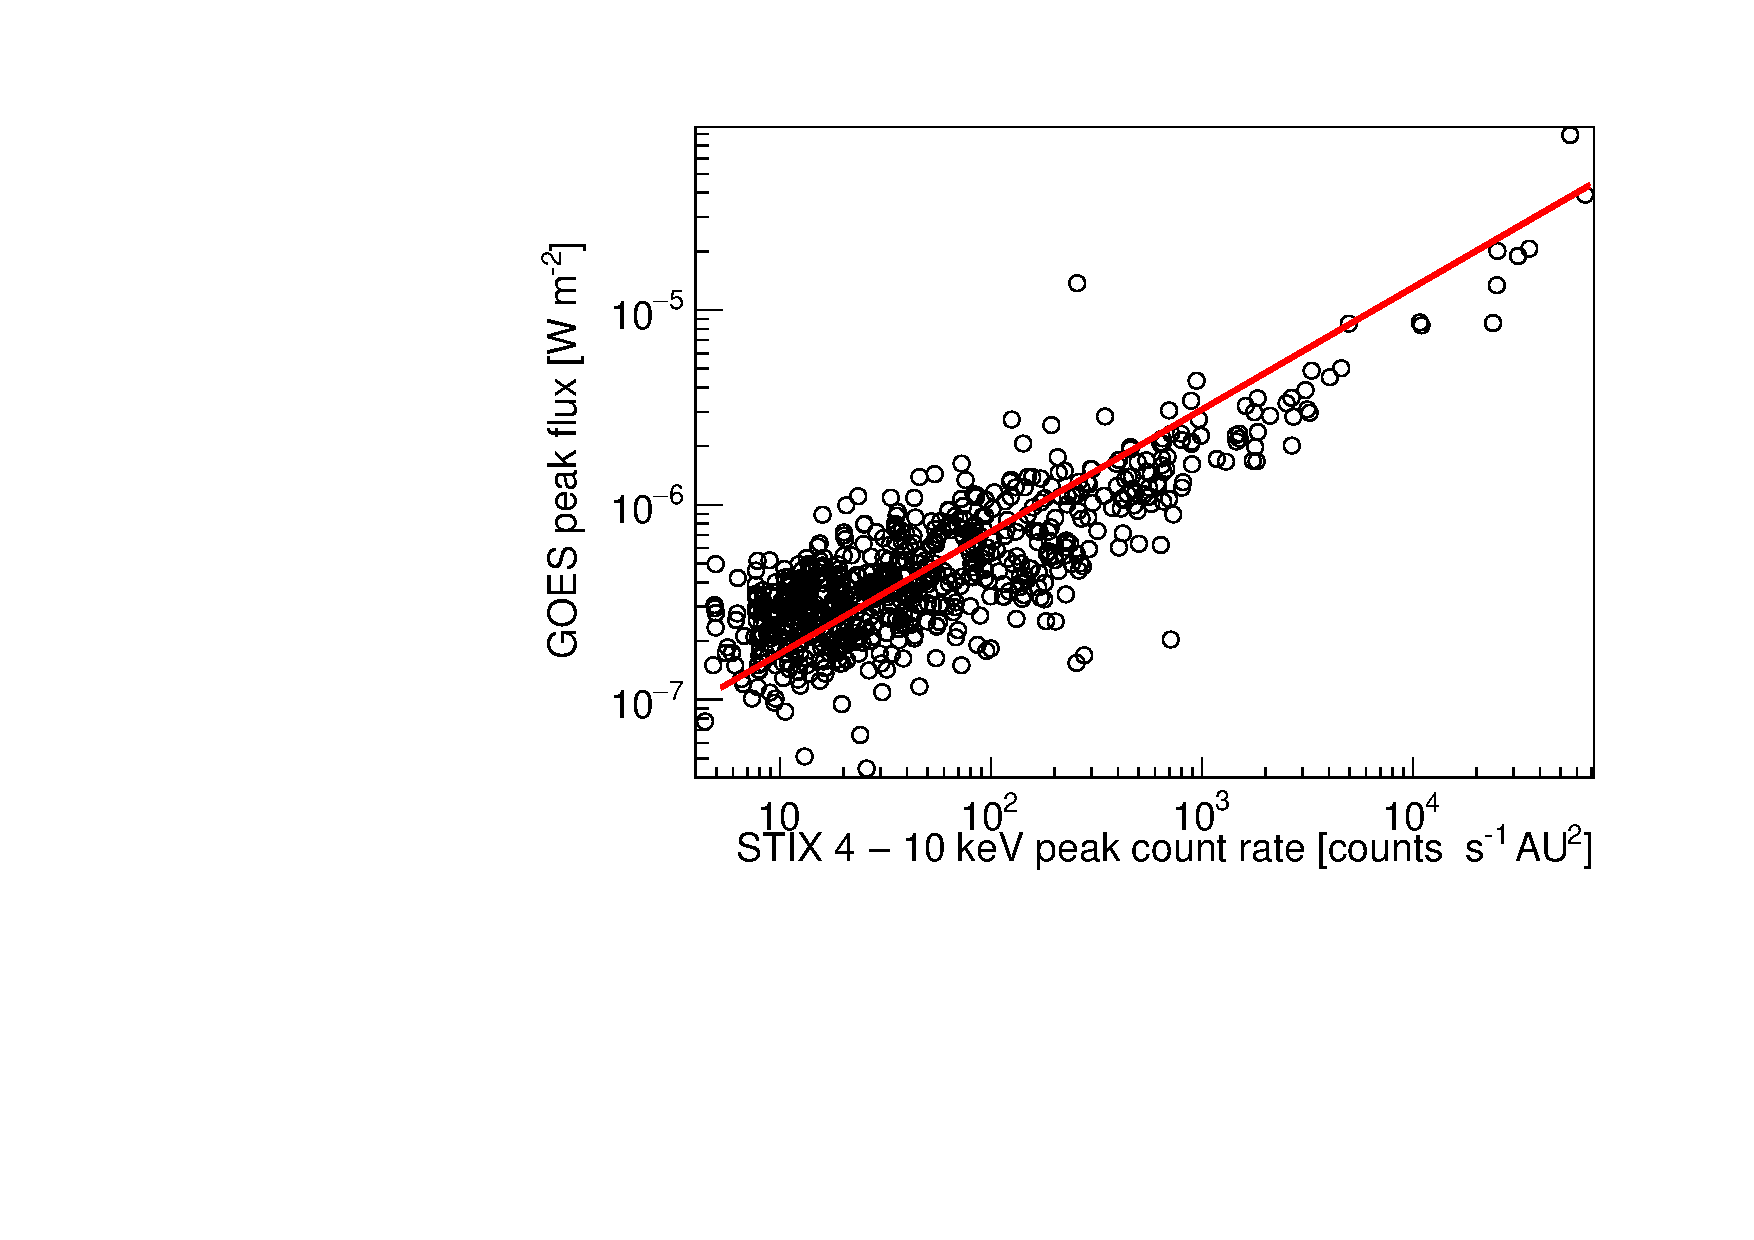
\includegraphics[width=0.8\linewidth]{figures/goes_stix_flux_paper.pdf}
  \caption{Scatter plot of GOES low channel peak flux with respect to STIX 1-AU equivalent  peak count rate in the 4 -- 10 keV range
  for 717 solar flares observed by both GOES and STIX duration the commissioning phase. 
  The solid line is a linear fit to the log-log graph. 
From the fit, we obtained 
the GOES flux in units of W/m$^2$ $\log_{10}(f) = 0.622 -7.376 \log_{10} (x^{'})$,
where $x^{'}$ is STIX
peak count rate corrected for the distance variations between the Sun and Solar Orbiter. 
%  The slope and 
%  interception for the best fit are $0.622\pm 0.002$ and $-7.376\pm0.067$, respectively.
%STIX count rate are background subtracted and corrected for the distance variations between the Sun and Solar Orbiter. 
}
\label{fig:goes-stix}
\end{figure}
It is straightforward to calculate the GOES
class of a flare observed by STIX from GOES flux if it is observed by GOES. 
However,  most of the time Solar Orbiter is far away from Earth and looks at 
the sun from different angles. Therefore a considerable number of flares observed by STIX
 are not observed by near earth satellites (and vice verse). 
As already discussed in Ref.~\cite{andrea2021}, 
it is possible to estimate GOES classes by using STIX count rates.
In order to study the correction, we selected 717 solar flares observed by 
by both GOES  and   STIX during the commissioning phase.   
Fig.~\ref{fig:goes-stix} shows the scatter plot of GOES low channel peak flux with respect to 
STIX peak count rate  of the 4 -- 10 keV QL light curves. 
STIX count rates  have been subtracted for background,  and corrected for 
the difference distance of Solar Orbiter to the Sun using $x^{'}=x r^2$, where $x$ is the count rate after background subtraction
 and $r$ the distance between Solar Orbiter and the Sun. 
As can be seen in the figure, there is clear correlation between
these two quantities.  The wide spread at the low flux could be explained by the difference in 
the energy response of the two instruments and in the flare temperatures. 
A linear line was fitted to the  correlation in the log-log scale. 
From the fit, we obtained 
the GOES flux in units of W/m$^2$ $\log_{10}(f) = 0.622 -7.376 \log_{10} (x^{'})$.
%where $x^{'}$ is STIX
%peak count rate corrected for the distance variations between the Sun and Solar Orbiter. 
The formula is currently used to estimate GOES classes  of flares observed by STIX. 
It is  worthwhile to mention that more observations will be included into the fit.
The estimated GOES classes as well as those from GOES measurements 
are stored in the flare list database. 

\subsubsection{Coarse flare location estimation}
Flare centroid location can constraint flaring region when reconstructing flare images.
STIX uses a dedicated sub-collimator called Coarse Flare Locator (CFL) to estimate flare locations.
The CFL consists of a front grid with
a distinctive pattern which selectively illuminates pixels of a 
dedicated detector based on the source location.
Flare location is estimated onboard by maximizing the correlation between observed CFL pixels counts 
with expected counts using a look-up table. 
However, due to the constraints of onboard computation, the onboard flare location is  only calculated for intermediate flares 
and has an accuracy of about 2 arcmin. 
With the downloaded measured counts  in each pixel,
the coarse flare location can be reconstructed to on the ground as well. 
This allows for more sophisticated algorithms, greater flexibility of selecting time and energy 
range to be integrated, and more careful background subtraction.

\begin{figure*}
  \centering
  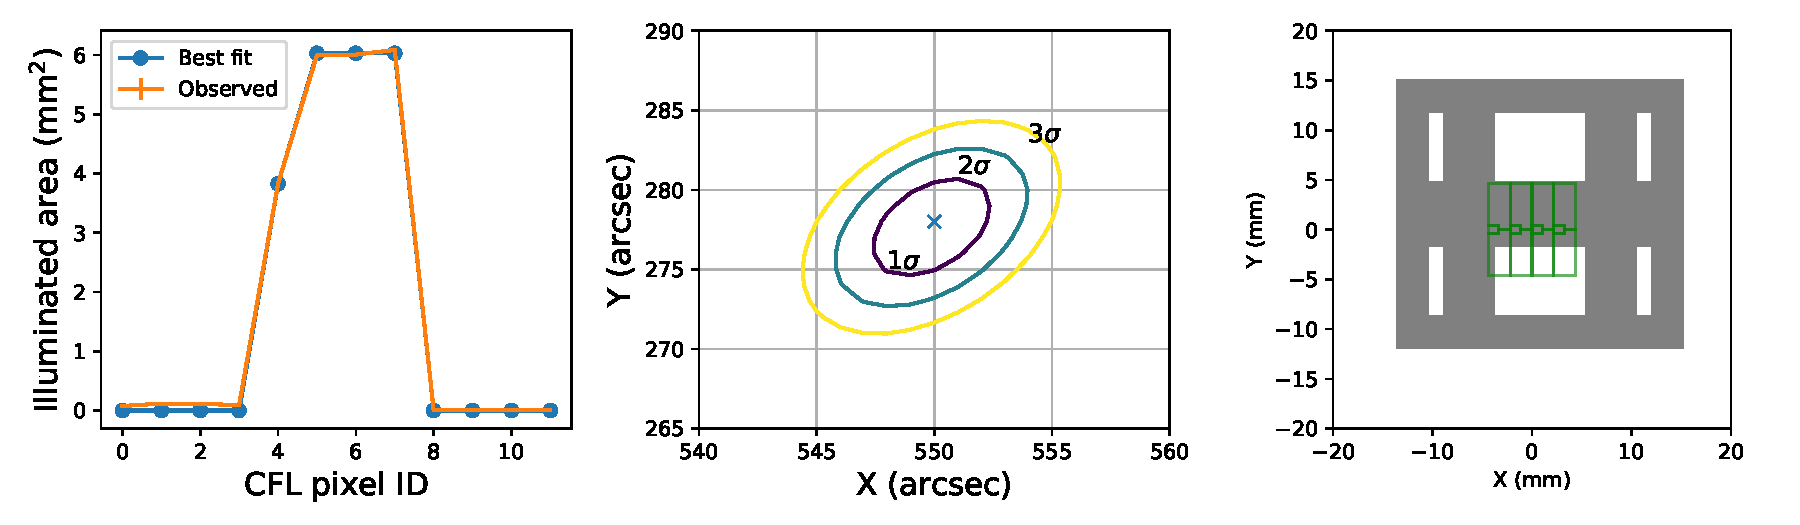
\includegraphics[width=0.95\linewidth]{figures/cflMay07.pdf}
  \caption{
   Left: Areas of illuminated regions of 12 pixels calculated by combining
  the twelve pixels counts with averages from other detectors, and the best fit. 
  Pixels 0 -- 3 are the top big pixels, Pixels 4 -- 7 are the bottom pixels and 8 -- 11 the small pixels as shown in the right panel.
   Middle: Best-fit flare centroid location (marked by x) and its 1$\sigma$, 2$\sigma$ and 3$\sigma$ confidence contours.
   The best-fit location is obtained at (550, 278) sec. 
    Right:  Shadow (the grey shaded regions) of CFL sub-collimator projected on the detector 
  for the best-fit flare location. }
  \label{fig:cfl}
\end{figure*}

The coarse location of an observed flare is estimated on ground after its pixel data (onboard level-1) is parsed.
The procedure consists of the following steps:
\begin{itemize}
  \item Selection of pixel data based on the flare time range and energy range information stored in the flare list dataset;
  \item Subtraction of background. The most recent level-1 dataset for the quiet sun period is used for background subtraction;
  \item Calculation of the mean fluence except for the CFL and the background detectors; 
      Except for the those two detectors, the ratio between the illuminated area and total area $r$ only depends on the 
      slit width and the pitch width. It doesn't vary with the position of the flare in the STIX FOV.  
      Therefore, the fluence of a detector can be given by $F=c/(r S_{\rm d})$,  where $c$ is the registered 
      count and $S_\textrm{det}$ the sum of the sensitive areas of twelve pixels. 
  \item Calculation of the areas of illuminated regions on CFL pixels $\vec{S}$ using $\vec{S} = \vec{C}/F$, where $C$  is an array of counts 
  recorded by 12 pixels. Their errors of the areas are also calculated; 
  \item  Coarse flare location is estimated by minimizing the weighted sum of squared deviations 
  (i.e. weighted chi-squares) between  the calculated illuminated areas and  expectations
  simulated for potential flare locations in a 400 $\times$ 400 grid, whose locations are separated by 10 arcsec.  
  \item Saving the calculated flare location to the flare list dataset. 
\end{itemize}
As an example, the left panel of Fig.~\ref{fig:cfl} shows the calculated and best-fit illuminated areas 
of the CFL pixels measure observed for STIX flare 2105071900 (GOES class M3.9);   the middle panel shows the best-fit 
flare centroid location, as well as its $1\sigma$, $2\sigma$ and $3\sigma$ contours. 
The simulated shadow of the CFL sub-collimator  is shown in the right panel. 
%\subsubsection{Joint observation}

\subsubsection{Image reconstruction and spectral analysis}
\begin{figure*}
  \centering
  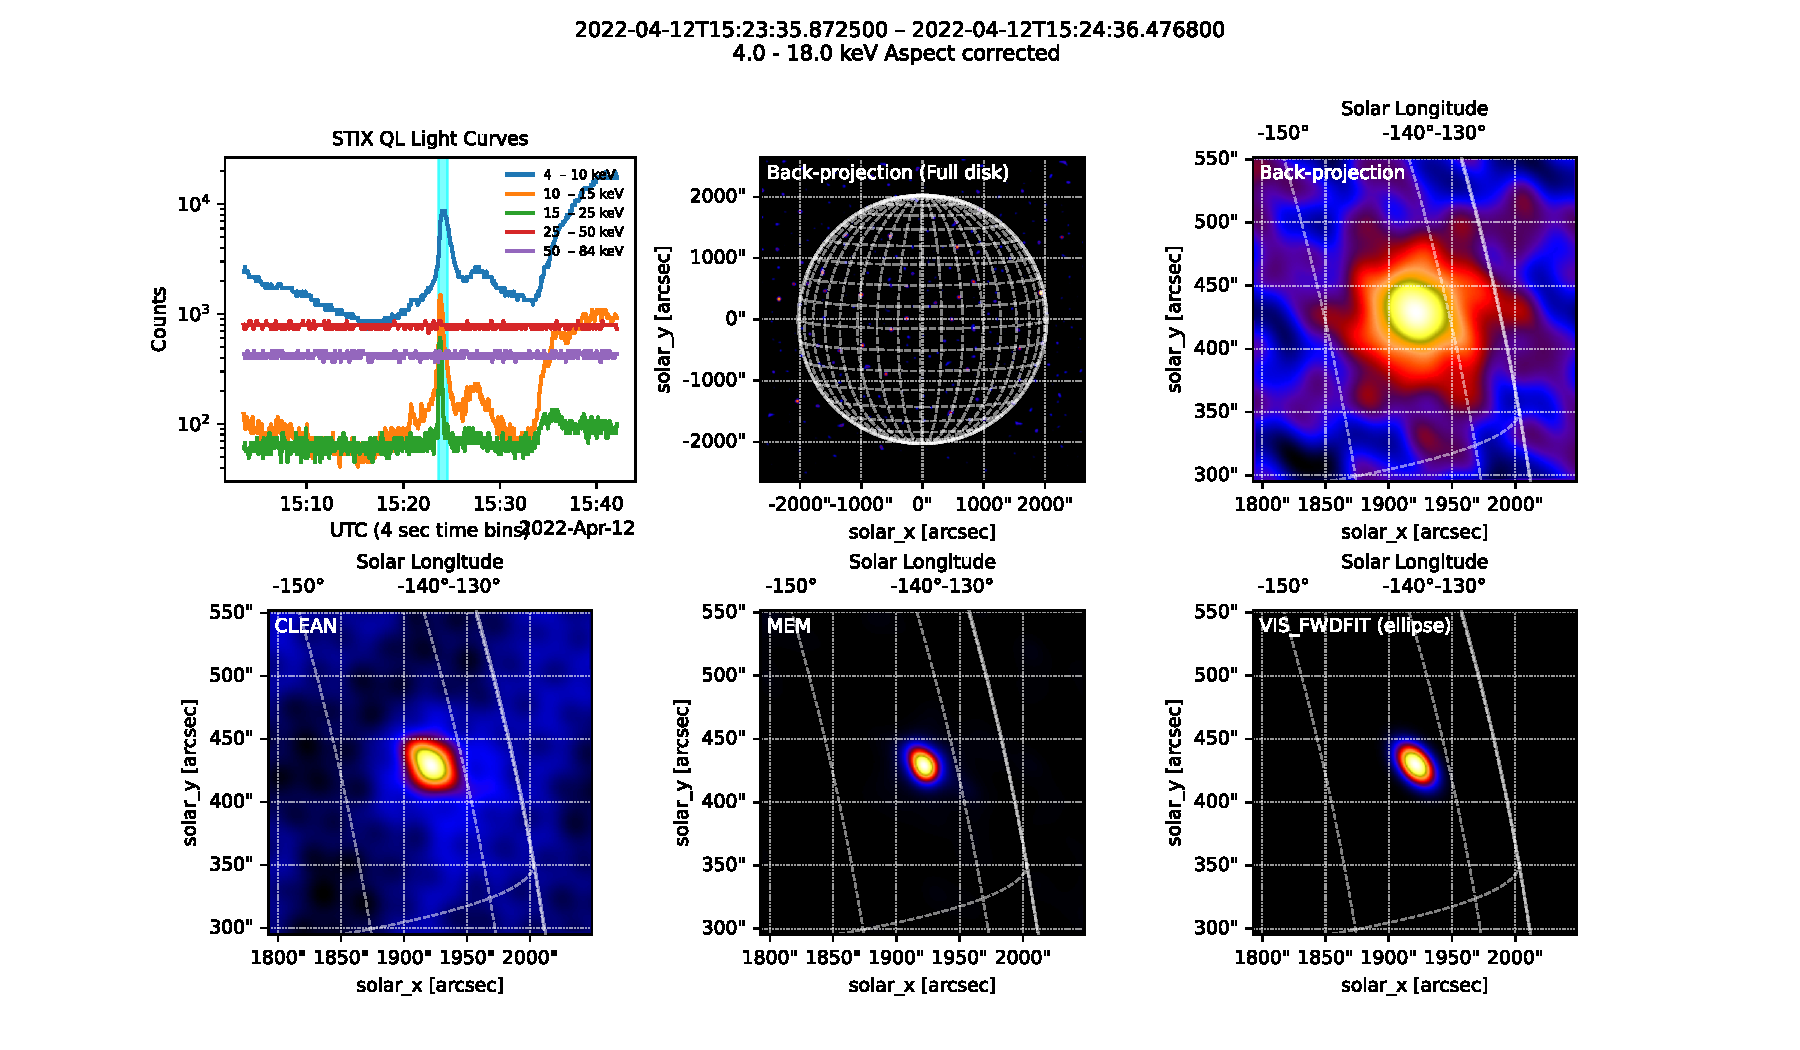
\includegraphics[width=0.95\linewidth]{figures/imaging_pipeline.pdf}
  \caption{ 
   STIX Quick-look light curves and reconstructed images of the solar flare observed at 2022-03-08T08:55:17Z, 
   created by the image reconstruction pipeline.  The time period at the peak was selected and 
   Back-projection, CLEAN, EM and VIS\_FWDFIT algorithms were used for reconstructing images. Image products are accessible
   at STIX data center.}
  \label{fig:imaging}
\end{figure*}
STIX detects thousands of  solar flares each year. However, only
 a part of them are analyzed in detail by solar physicists. 
To facilitate the selection of flares of interest, a flare imaging reconstruction and spectral fitting pipeline 
has been developed and integrated into the main data processing pipeline on the platform. 
For each flare, pixel counts recorded within one-minute time frame around the flare peaks  
are selected.
Reconstruction of an image require inputs such as background data in the same level, 
STIX pointing information, spacecraft orientation. 
They are prepared based on the knowledge in the NoSQL. 
After background subtraction, transmission and dead time corrections, the selected counts are used for 
calculation of visibilities for two energy ranges 4 -- 10 keV (thermal emission) and 16 -- 28 (non-thermal)  
keV.
Then images are reconstructed with four different algorithms: Back-projection, CLEAN, 
MEM and VIS\_FWDFIT \cite{paolo2020,clean,mem}.
Reconstructed images are further corrected for STIX off-pointing and spacecraft rotations with the auxiliary data. 
As an example,  the first panel of Fig. ~\ref{fig:imaging} shows 
the light curves and time range selected for a flare occurred at about 2022-03-08T08:55:17Z .
The rest of the panels show the reconstructed images. 
The final by the pipeline are written to files in FITS  and PNG formats, while
their metadata are written to the NoSQL database.  
%They are accessible from STIX data center website or via stixdcpy\footnote{stixdcpy}.
\subsubsection{Spectral analysis}
Energy spectra provide direct information on electron acceleration in solar flares. 
The x-ray spectral fitting package OSPEX in SSWIDL includes a wide range of commonly used functions for parametrising the thermal
and non-thermal components as well as an interface to perform
the fits \footnote{\url{https://hesperia.gsfc.nasa.gov/ssw/packages/spex/doc/}}.
It reads pixel count data from L1 FITS files, corrections for dead time, transmission and energy binning for the counts,  
and calls  OSPEX routines for spectral fitting. 
\begin{figure}
  \centering
  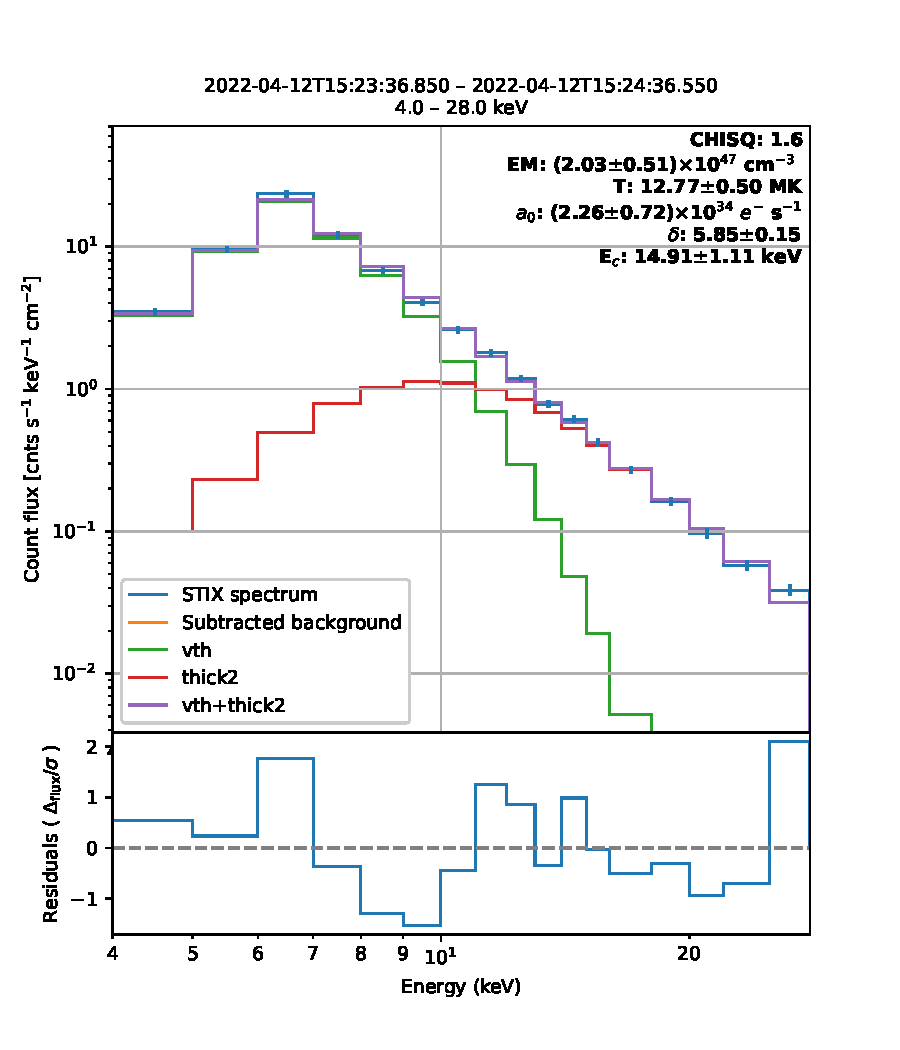
\includegraphics[width=0.9\linewidth]{figures/ospex.pdf}
  \caption{ 
    An example of spectral fitting results . The imaging and spectroscopy pipeline performs
    spectral analysis for all flares in the flare list. Spectral fitting results are written to both FITS files and 
    the NoSQL database.
   }
  \label{fig:ospex}
\end{figure}
\section{Requesting Science data}
STIX only down-links low-latency data 
automatically due to the data rate constraints.  
Pixel data with higher time and energy resolution contain much richer information. 
They persist in the onboard archive memory for about five to six months 
before they are overwritten.
They can be compressed and 
down-linked  after receiving data request telecommands initiated  by the STIX operation team. 
A data request telecommand needs to provide information on the
time range, minimal time binning, energy range, energy binning  and selected detectors (or pixels), based on 
the knowledge from low-latency quick-look light curves.
Requesting science data from STIX is a tedious task, as it must take
into account many factors, such as constraints on the  allocated telemetry data rate, 
the daily maximum number of requests that can be submitted,  
the onboard time binning, 
solar flare fluxes and the scientific value of the data. 
After two years of operation, the following data selection strategy has been adopted: 
\begin{itemize}
  \item 
  Level-1 pixel data 
  of the flaring time period is requested for detected flares with a total number signal counts  greater than 1000, 
  which is  the minimal counts to reconstruct an image.  
  In order to minimize the telemetry data size, 
  the energy range of the request is limited to the range with signal counts based on the 
  knowledge from light curves. 
  If the pixel-summed peak count rate is less than 125 counts/sec
  (equivalent to the count rate observed for a B3 flare at 1 au), 
  a single time-bin is requested. Otherwise, a finer time resolution of science data is requested.
  The actual time resolution is adjusted based on the amount of data allocated.
 \item Spectrograms (onboard level-4) require relative small amount data, therefore
  the highest possible time resolution (~ 0.5 seconds depending on the configuration)
   and energy resolution  (no rebinning of science energy bins) are requested for all time periods that STIX is in NOMINAL mode. 
\item At least one level 1 scientific data background data is requested per day. 
Background period selection is done by excluding periods from the list of flares stored in the database. 
If a quiet solar period is not found, a relatively quiet solar period will be selected. To reduce the amount of telemetry data, 
background data request counts are time-integrated over the requested time period, i.e., a single time-bin.
\end{itemize}
A routine has been developed to create data requests mentioned above automatically. 
An unique ID is assigned to each request.
Unique IDs have a format of {\em yymmddxxxx}, where 
the first eight digits indicate the two-digit year,  month, day of the data start time, respectively, 
and the last four digits are a random number, which is unique for the day.  
Information of created data requests is stored in the NoSQL database. 
After being checked by STIX team, data requests  are flagged as pending requests.
Then they are selected compiled to instrument operation requests (IORs), which are used to create the final telecommands
to be executed by the instrument.
Apart from those automatically created data requests, 
data requests are also created by the instrument team for special requirements.
\section{STIX data center interfaces}

\begin{figure*}[h]
  \centering
  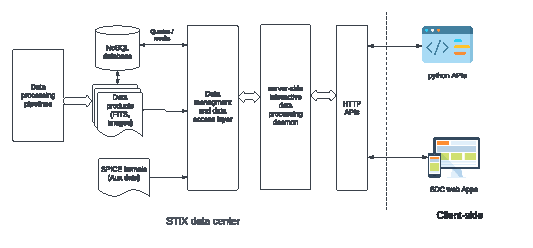
\includegraphics[width=0.6\linewidth]{figures/interfaces.pdf}
  \caption{ 
    STIX data center client-side and server-side data exchanging mechanisms.
   }
  \label{fig:interfaces}
\end{figure*}



Being aware of the complex structure of STIX data and the wide variety of 
data products types,  we developed Web APIs to facilitate querying and accessing the data. 
Based on the http APIs, we have developed web-based interfaces, 
and application interfaces for python and IDL. 
\subsection{Web-based graphical interfaces}
Web applications are accessible with a web browser anywhere, and can eliminate 
compability issues.   We have developed tens of web-based applications with modern web techniques. 
Fig. \ref{fig:interfaces}




They are available at STIX data center website\footnote{https://datacenter.stix.i4ds.net/}.
Data products and metadata generated by STIX data center are either 
written to files to  
Web-based applications are selected for the graphical
 interfaces at the data center. 
 This process enables the advantages 
 of clear cross-platform usability and wide access for internet browsers. 
 As an example, Fig. 4 shows the web-based light curve viewer mentioned in Section 8.1.
 The client side and server side interact and operate as shown in Fig. 
  The details are given below:

STIX data center provides web data browsers to all L1 data, auxilary data , which include 
- housekeeping data browser.  housekeeping data can be 
- Science data browser

It provides  the capability to perform customized analysis with state-of-art methods without installating software or download raw data.
THe platform runs on the computing infrastructure at FHNW and 
it provides  the capability to perform customised 
analysis with state-of-art methods without installating software or download raw data.
The barried to explore stix data is greately reduced for newcommers. The
access is facilitated for experienced users.

One can obtain images, spectra and light curves from the web interface for a large dataset. 



Caching, balencing and preprocessing
\subsection{Data access}
\subsection{Data query APIs}
Calibration data products
https://fermi.gsfc.nasa.gov/ssc/data/access/gbm/
\section{Tools for scientitic analysis }
\subsection{Data access and APIs}
\label{sec:apis}
stixdcpy allows you to query and download data which are available at STIX data center, include
Quick-look light curves
Housekeeping data
Science data
\subsection{Service for web based analysis}
SWAN (Service for Web based ANalysis)
 is a platform to perform interactive data analysis in the cloud.
Analyse data without the need to install any software
data archive. 
There are minjnor difference between the data in L1 and 
FITS files are split for low latency data 

In most cases, three platforms contains the same data. 
Information metadata might be slightly different 

May often be produces 
\section{Imaging and spectroscopy service}

\section{Summary}
\label{sec:summary}



% WARNING
%-------------------------------------------------------------------
% Please note that we have included the references to the file aa.dem in
% order to compile it, but we ask you to:
%
% - use BibTeX with the regular commands:
%   \bibliographystyle{aa} % style aa.bst
%   \bibliography{Yourfile} % your references Yourfile.bib
%
% - join the .bib files when you upload your source files
%-------------------------------------------------------------------

\bibliographystyle{aa}
\bibliography{citations}

\end{document}
